\section{Auswertung}
\label{sec:Auswertung}
\subsection{Strahlungsleistung als Funktion der Temperatur und Bestimmung des Emissionsvermögens}
Die zu Beginn des Versuchs gemessene Offsetspannung beträg $U_0=0.0062 \,\si{\milli\volt}$.
Da die Ansprechzeit der verwendeten Geräte sehr gering ist, entfällt die Messung
der Anprechzeit der Themosäule.
Es werden die Thermospannungen für die vier Oberflächen des Leslie-Würfels als
Funktion der Temperatur gemessen, nachdem die Temperatur von der Anfangstemperatur
$T_\symup{max}=365.85 \si{\kelvin}$ um je weitere $5 \si{\kelvin}$ gefallen ist.
In Tabelle \ref{tab:thermospannungen} sind die gemessenen Werte für die Temperatur
und die Thermospannung dargestellt.
\begin{table}
  \centering
  \begin{tabular}{c c c c c}
    \toprule
    Temperatur T in \si{\kelvin} & \multicolumn {4}{c}{Thermospannung U in \si{\milli\volt}}\\
    & schwarz & glänzend & \;weiß & \quad matt \\
    \midrule
     365.85 & 1.031 & 0.072 & \; 0.992 & \quad 0.172 \\
     360.85 & 0.958 & 0.071 & \; 0.895 & \quad 0.156 \\
     355.85 & 0.856 & 0.065 & \; 0.816 & \quad 0.151 \\
     350.85 & 0.761 & 0.060 & \; 0.732 & \quad 0.138 \\
     345.85 & 0.666 & 0.051 & \; 0.639 & \quad 0.107 \\
     340.85 & 0.580 & 0.039 & \; 0.552 & \quad 0.101 \\
     335.85 & 0.503 & 0.031 & \; 0.476 & \quad 0.081 \\
     330.85 & 0.428 & 0.028 & \; 0.408 & \quad 0.069 \\
     325.85 & 0.353 & 0.030 & \; 0.333 & \quad 0.064 \\
     320.85 & 0.278 & 0.019 & \; 0.271 & \quad 0.058 \\
     315.85 & 0.210 & 0.018 & \; 0.199 & \quad 0.039 \\
     310.85 & 0.149 & 0.019 & \; 0.145 & \quad 0.036 \\
    \bottomrule
  \end{tabular}
  \caption{Thermospannungen in Abhänigkeit der Temperatur und Oberfläche.}
  \label{tab:thermospannungen}
\end{table}

Die erneut gemessene Offestspannung ergibt nach Ende der Messreihe einen Wert von
$U_0=0.0081 \,\si{\milli\volt}$. Der Mittelwert der Offsetspannung, der nach
\begin{equation}
  \bar{x} = \frac{1}{N} \sum_{\symup{i}=1}^{N} x_\symup{i}
  \label{eqn:mittelwert}
\end{equation}

berechnet wird, ergibt sich zu $\bar{U_0} = 0.0072 \,\si{\milli\volt}$.
Die Thermospannung wird als Funktion von $T^4 - T_0^4$ aufgetragen, wobei $T_0 = 294,15 \si{\kelvin}$
die Raumtemperatur ist.
Mit $U_0$ und $T_0$ lassen sich die Werte $T^4-T_0^4$ und $U-U_0$ für die verschiedenen
Oberflächen berechnen, welche in Tabelle \ref{tab:rechenwerte} aufgeführt und in
der Abbildung \ref{fig:thermospannung} graphisch dargestellt sind.
\begin{table}
  \centering
  \begin{tabular}{c c c c c}
    \toprule
    Temperatur $T^4-T_0^4$ in \si{10^{10}\kelvin^4} & \multicolumn {4}{c}{Thermospannung $U-U_0$ in \si{\milli\volt}}\\
    & schwarz & glänzend & \;weiß & \quad matt \\
    \midrule
     1.792  &  1.024  &  0.065  &  0.985  &  0.165 \\
     1.696  &  0.951  &  0.064  &  0.888  &  0.149 \\
     1.603  &  0.849  &  0.058  &  0.809  &  0.144 \\
     1.515  &  0.754  &  0.053  &  0.725  &  0.131 \\
     1.431  &  0.659  &  0.044  &  0.632  &  0.998 \\
     1.350  &  0.573  &  0.032  &  0.545  &  0.938 \\
     1.272  &  0.496  &  0.024  &  0.469  &  0.738 \\
     1.198  &  0.421  &  0.021  &  0.401  &  0.618 \\
     1.127  &  0.346  &  0.023  &  0.326  &  0.568 \\
     1.060  &  0.271  &  0.012  &  0.264  &  0.508 \\
     0.995  &  0.203  &  0.011  &  0.192  &  0.318 \\
     0.934  &  0.142  &  0.012  &  0.138  &  0.288 \\
    \bottomrule
  \end{tabular}
  \caption{Berechnete Werte für $T^4-T_0^4$ und $U-U_0$ für alle Flächen.}
  \label{tab:rechenwerte}
\end{table}
\begin{figure}
  \centering
  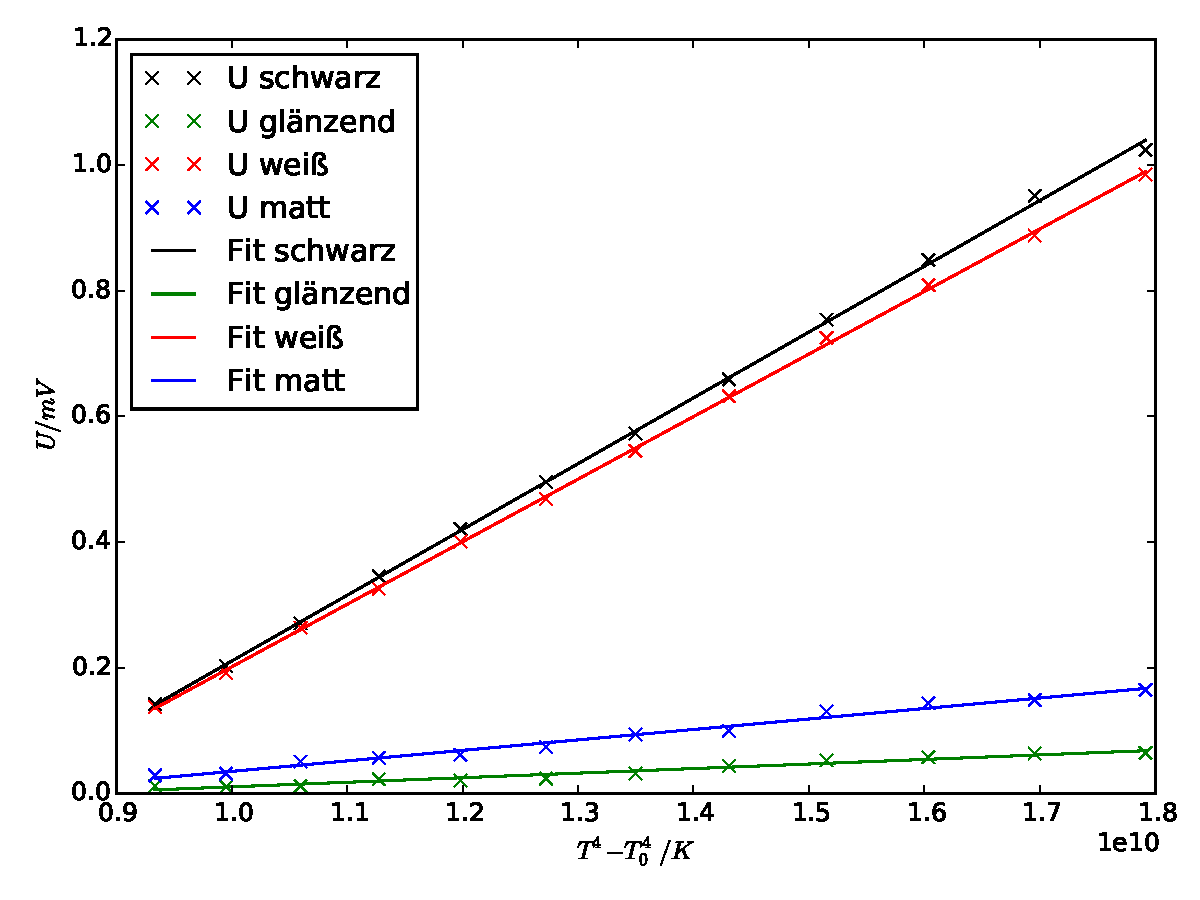
\includegraphics[width=0.82\textwidth]{thermospannung.pdf}
  \caption{Messwerte und Fits für die Thermospannung in Abhängigkeit von \mbox{$T^4 - T_0^4$.}}
  \label{fig:thermospannung}
\end{figure}
\newline
Die Fits werden mit linearer Regression der Form $f(x) = a \cdot x + b $ mit Python
berechnet.
Für die Parameter ergeben sich folgende Werte:
\begin{align*}
  a_\symup{schwarz}   &= \,(1.047\pm0.007)\cdot10^{-10} \si{\frac{\volt}{\kelvin^4}} \\
  b_\symup{schwarz}   &= (-0.84\pm0.01) \si{\volt} \\
  a_\symup{glaenzend} &= \,(7.3\pm0.5)\cdot10^{-12} \si{\frac{\volt}{\kelvin^4}} \\
  b_\symup{glaenzend} &= (-0.062\pm0.006) \si{\volt} \\
  a_\symup{weiss}     &= \,(9.95\pm0.06)\cdot10^{-11} \si{\frac{\volt}{\kelvin^4}} \\
  b_\symup{weiss}     &= (-0.794\pm0.008) \si{\volt} \\
  a_\symup{matt}      &= \,(1.67\pm0.07)\cdot10^{-11} \si{\frac{\volt}{\kelvin^4}} \\
  b_\symup{matt}      &= (-0.131\pm0.009) \si{\volt}
\end{align*}
Es wird nun angenommen, dass die schwarze Oberfläche ein schwarzer Strahler ist
und demnach $\epsilon_\symup{schwarz} = 1$ gilt.
Dann lassen sich die Emissionsvermögen der anderen Oberflächen wie folgt berechnen:
\begin{equation}
  \epsilon_\symup{i} = \frac{a_\symup{i}}{a_\symup{schwarz}},
  \label{eqn:epsilon}
\end{equation}
und man erhält als Ergebnis für die Emissionsvermögen $\epsilon_\symup{i}$:
\begin{align*}
  \epsilon_\symup{schwarz}   &= 1 \\
  \epsilon_\symup{glaenzend} &= (0.069\pm0.004) \\
  \epsilon_\symup{weiss}     &= (0.951\pm0.009) \\
  \epsilon_\symup{matt}      &= (0.159\pm0.006).
\end{align*}
Der Fehler berechnet sich dabei nach der Gaußschen Fehlerfortpflanzung
\begin{equation}
  \Delta f(x_\symup{i}) = \sqrt{\sum_{\symup{i}=1}^N
  \left(\frac{\partial f}{\partial x_\symup{i}}\right)^2 \cdot
  (\Delta x_\symup{i})^2}
  \label{eqn:gaussfehler-allgemein}
\end{equation}
für Funktionen mit den fehlerbehafteten Größen $\Delta x_\symup{i}$.
Der Gaußfehler der Gleichung \eqref{eqn:epsilon} wird mit
\begin{equation}
  \Delta \epsilon_\symup{i}(a_\symup{i},a_\symup{s}) =
  \sqrt{\left(\frac{1}{a_\symup{s}}\right)^2\cdot(\Delta a_\symup{i})^2
  + \left(\frac{a_\symup{i}}{{a_\symup{s}}^2}\right)^2
  \cdot(\Delta a_\symup{s})^2}
  \label{eqn:gaussfehler-epsilon}
\end{equation}
berechnet. Dabei entspricht $a_\symup{s}$ $a_\symup{schwarz}$.

\subsection{Strahlungsleistung als Funktion des Abstands}
In einer weiteren Messreihe werden die Thermospannungen bei konstanter Temperatur
$T=320.25\si{\kelvin}$ und veränderlichem Abstand für die schwarze Oberfläche
gemessen. Die Ergebnisse sind in Tabelle \ref{tab:thermospannung2} dargestellt.
\begin{table}
  \centering
  \begin{tabular}{c c}
    \toprule
    Abstand x in cm & Thermospannung U in \si{\milli\volt}\\
    \midrule
    10 & 0.269  \\
    11 & 0.264  \\
    12 & 0.260  \\
    13 & 0.2530 \\
    14 & 0.2474 \\
    15 & 0.2426 \\
    16 & 0.2373 \\
    17 & 0.2301 \\
    18 & 0.2236 \\
    19 & 0.2176 \\
    20 & 0.2108 \\
    \bottomrule
  \end{tabular}
 \caption{Thermospannungen der schwarzen Fläche\\in Abhänigkeit des Abstands.}
 \label{tab:thermospannung2}
\end{table}
\newpage
Als grafische Darstellung erhält man mit den Fitparametern c und d für die
\begin{figure}
  \centering
  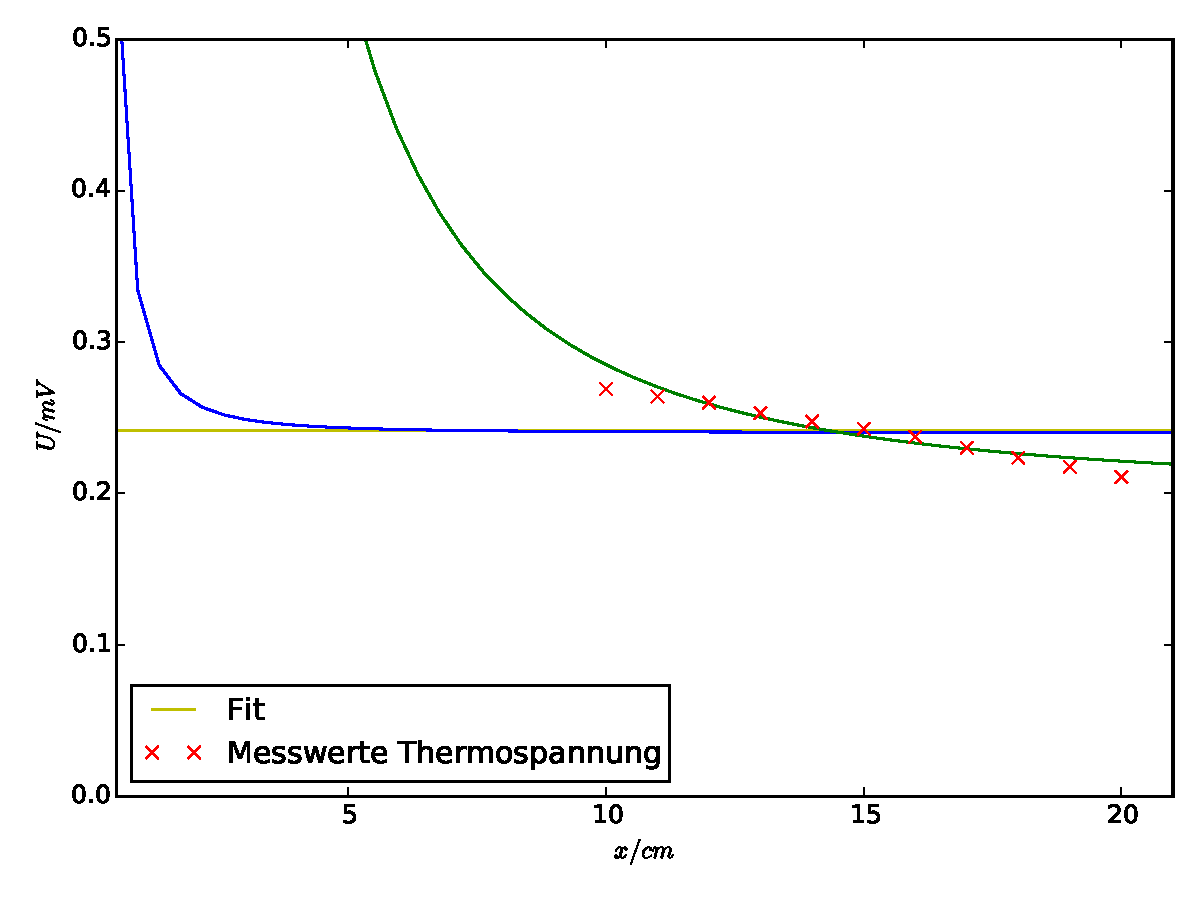
\includegraphics[width=0.9\textwidth]{strahlintensitaet.pdf}
  \caption{Strahlenintensität in Abhängigkeit des Abstands.}
  \label{fig:strahlintensitaet}
\end{figure}
Regression der Form $f(x) = \frac{c}{x^2} + d $ einen Fit, wie er in Abbildung
\ref{fig:strahlintensitaet} zu sehen ist. Man erhält durch einen Fit mit Gnuplot
folgende Parameter:
\begin{align*}
  c &= (7.543\pm0.874) \si{\frac{\milli\volt}{\centi\meter}} \\
  d &= (0.203\pm0.005) \si{\milli\volt}.
\end{align*}
